This section presents the final TRITIUM monitor. A schematic design is shown in Figure \ref{fig:TritiumDetectorSchematicDesign}.

\begin{figure}[h]
\centering
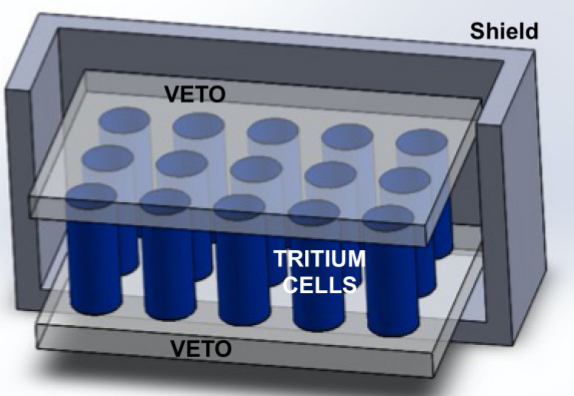
\includegraphics[scale=0.5]{5Prototypes/55ModularTritiumDetector/FinalTritium.png}
\caption{A schematic design of the TRITIUM detector.\label{fig:TritiumDetectorSchematicDesign}}
\end{figure}

It consists of a number of TRITIUM modules read in parallel. Each module is the prototypes that achieves better results, TRITIUM-Aveiro or TRITIUM-IFIC 2. These modules are shielded from environmental radioactivity by three different techniques:

\begin{enumerate}

\item{} An external lead shielding, which is used to stop the environmental radioactivity and soft cosmic rays (particles with energies below $200~\MeV$).

\item{} Several active vetos, which is placed below and above the TRITIUM modules. These active vetos are read in anticoincidence to supress high energy event background, mainly cosmic ray particles with energies above $200~\MeV$.

\item{} The radioactive elements present in the water samples, measured by the TRITIUM monitor, are eliminated by the ultrapure water system.

\end{enumerate}

The ultrapure water system, the lead shielding and a TRITIUM-Aveiro prototype are installed and currently in operation at the Arrocampo dam. This entire system is employed to successfully monitor the tritium levels in Arrocampo dam during several months. Furthermore, two additional TRITIUM-Aveiro prototypes and four active vetos are currently under construction and will be measured in parallel with this prototype.

The electronics of the TRITIUM-Aveiro prototype, based on a RaspberryPi, cannot be used for multiple modules due to counting limitations and this must be replaced by an FPGA-based counter board.

Simultaneously, three TRITIUM-IFIC 2 prototypes and an active veto are already built and they will be installed as soon as possible.

One of the most important aspects of the TRITIUM monitor is its modular design, which allows scalability to reach the required sensitivity, $100~\becquerel/\liter$. It means that if this target sensitivity is not reached with the three modules to be installed, may be obtained by installing additional modules.

The only scalability restriction is the available space, which is set by the lead shield already built and the cabin in which the setup is installed. The currently available space fit five different structures as the one shown in Figure \ref{fig:TritiumMonitorIFIC2Design}, each one containing 10 modules and one active veto. If all the 50 TRITIUM modules are installed the sensitivity of the TRITIUM monitor could be improved a factor of around 7 ($\sqrt{50}$) with the respecto to the sensitivity of a single module.

\begin{figure}[h]
\centering
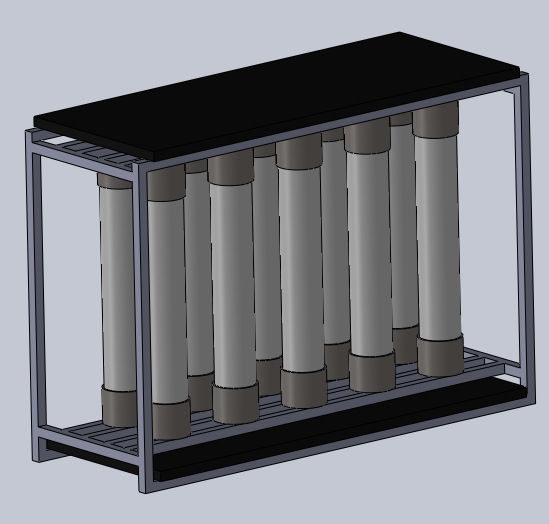
\includegraphics[scale=0.6]{5Prototypes/55ModularTritiumDetector/Tritium_Detector_Based_On_Tritium_IFIC_2.PNG}
\caption{A TRITIUM monitor design based on the TRITIUM-IFIC 2 prototype.\label{fig:TritiumMonitorIFIC2Design}}
\end{figure}